\documentclass[12pt,a4paper]{article}

\usepackage[T1]{fontenc}
\usepackage[utf8]{inputenc}
\usepackage[english]{babel}
\usepackage{geometry}
\geometry{top=2.5cm, bottom=2.5cm, left=2.5cm, right=2.5cm}
\usepackage{graphicx}
\usepackage{float}
\usepackage{subcaption}
\usepackage{booktabs}
\usepackage{tabularx}
\usepackage{listings}
\usepackage{xcolor}
\usepackage{hyperref}
\hypersetup{colorlinks=true, linkcolor=blue, citecolor=blue, urlcolor=blue}
\usepackage{setspace}
\usepackage{parskip}
\usepackage{microtype}
\usepackage{enumitem}
\usepackage{amsmath}
\usepackage{fancyhdr}
\pagestyle{fancy}
\fancyhf{}
\rhead{\small IRIS 2026 Hackathon}
\lhead{\small Br\"{u}ne, Corazza, Longo, Sapienza, Vagnoni}
\cfoot{\thepage}
\renewcommand{\headrulewidth}{0.4pt}

\onehalfspacing
\setlength{\parindent}{0pt}

\lstdefinelanguage{Turtle}{
  morekeywords={a,xsd,ex,legal,ipronto},
  morestring=[b]{"},
  morecomment=[l]{\#},
  sensitive=false,
}
\lstset{
  basicstyle=\footnotesize\ttfamily,
  keywordstyle=\color{blue!70!black}\bfseries,
  stringstyle=\color{brown},
  commentstyle=\color{gray}\itshape,
  breaklines=true,
  frame=single,
  framerule=0.4pt,
  rulecolor=\color{gray!40},
  backgroundcolor=\color{gray!5},
  aboveskip=6pt,
  belowskip=4pt,
}

% -----------------------------------------------------------------------
\title{
  \textbf{Bidirectional Monitoring of WIPO Regulation and National
  Legislation: A Neuro-Symbolic Approach}\\[0.6em]
}

\author{
  John Frederic Br\"{u}ne \quad Michele Corazza \quad Generoso Longo\\[0.2em]
  Salvatore Sapienza \quad Simone Vagnoni\\[0.4em]
  \small LAST-JD Programme, Universit\`{a} di Bologna, Italy\\[0.2em]
  \small Supervisor: Prof.\ Monica Palmirani
}

\date{May 2026}

% -----------------------------------------------------------------------
\begin{document}
{\singlespacing\maketitle}
\thispagestyle{fancy}

% ── Abstract ────────────────────────────────────────────────────────────
\begin{abstract}
\noindent
Checking whether national copyright law actually complies with WIPO
treaty obligations is still largely manual work. We built a
neuro-symbolic web application that does this automatically for nine
jurisdictions. A large language model handles the multilingual question,
and a knowledge graph built from Akoma Ntoso XML legal documents supplies
the answer. A user can ask in any language; the system finds the relevant
provision, links it back to the official source, and decides Berne
Convention compliance with no LLM in the loop. 
Beyond compliance assessment, the system provides two features aimed at practical legal research. First, every answer includes authenticated source attribution through links derived from FRBR metadata contained in the original legal documents. Second, the system supports point-in-time navigation across 68 historical versions of the Italian Copyright Act, allowing users to retrieve the version in force on a selected date. We manually validated all encoded copyright-duration values and resulting compliance classifications across the nine jurisdictions. Source code is at
\url{https://github.com/Stocastico96/ReMeP_Hackathon_26}.

\medskip
\noindent\textbf{Keywords:} neuro-symbolic AI, knowledge graph, Akoma Ntoso, copyright law, treaty compliance
\end{abstract}

\newpage

% ── 1. Introduction ─────────────────────────────────────────────────────
\section{Introduction}

WIPO coordinates intellectual property law through 28 treaties spanning
194 member states, yet there is limited automated support for systematically comparing national legislation against treaty obligations. Take a
question like ``Is the Italian \emph{Legge}~633/1941 compliant with
Article~7 of the Berne Convention?'' Answering it means a lawyer has to
find the right provision, read off its number (70~years \emph{post mortem
auctoris}), and hold that against the treaty floor of 50~years pma.
One country is tedious; doing it for nine by hand is slow and easy to get
wrong.

LLMs can read a legal query in any language, but they also invent
citations and numbers with some regularity~\cite{huang2023}. Knowledge
graphs have the opposite problem: they hold structured facts reliably,
yet they cannot make sense of a question phrased in Italian or French.
Our system puts each where it is strong. The LLM does the query
enrichment and writes the final answer; the knowledge graph retrieves
the legal evidence and runs the compliance check. The result is a
\textbf{neuro-symbolic} pipeline~\cite{hitzler2022} in which the
hallucination-prone part never touches the numbers a verdict depends on.

This paper describes a prototype we built for the IRIS 2026 Hackathon. At
its core is an end-to-end pipeline that carries a multilingual query
through LLM enrichment into SPARQL retrieval over an AKN-grounded IPROnto
knowledge graph, with a compliance checker that rests entirely on
integer-typed RDF triples and \texttt{ipronto:compliesWith} links and keeps
the LLM out of the actual decision. On top of that baseline, two features
do the work that makes the output usable in a legal setting. The first is
authentic source attribution: FRBR Work URIs and ELI identifiers, pulled
from the AKN \texttt{FRBRWork} metadata and surfaced in the UI as verifiable
links to the official legislative text. The second is point-in-time
navigation, which resolves any of the 68 historical AKN expressions of the
Italian copyright act (1941-2025) to whichever was in force on the date a
user asks about.

% ── 2. Background ───────────────────────────────────────────────────────
\section{Background and Related Work}

\subsection{Akoma Ntoso and the FRBR/ELI Model}

Akoma Ntoso (AKN) is the OASIS/UN standard for the XML representation of
legal and parliamentary documents, originally developed at the University
of Bologna~\cite{oasis2018,palmirani2011}. Its hierarchical element tree
(\texttt{<act>}, \texttt{<section>}, \texttt{<article>},
\texttt{<paragraph>}) assigns stable \texttt{eId} attributes to every
provision, which lets us cite at the paragraph level across versions and,
more importantly for a symbolic system, query a provision directly from its
structural metadata without parsing any natural language.

AKN embeds a FRBR metadata layer~\cite{ifla1998} encoding the
Work-Expression-Manifestation-Item hierarchy. The \texttt{<FRBRWork>}
element carries: \texttt{FRBRuri} (canonical Work-level URI);
\texttt{FRBRdate} (dated events typed by a \texttt{name} attribute, e.g.\
\emph{dateApplicability}, \emph{dateEntryInForce}); \texttt{FRBRalias}
(aliases, including the European Legislation Identifier,
ELI~\cite{eli2012}); and boolean flags \texttt{FRBRauthoritative} /
\texttt{FRBRprescriptive} marking official, legally binding sources.
In practice these fields are populated unevenly from one national corpus
to the next. For example: The UK uses \texttt{FRBRprescriptive}, Switzerland uses
\texttt{FRBRauthoritative}, and Germany sets neither. 

\subsection{IPROnto}

IPROnto is an OWL ontology for the IP domain developed by the Distributed
Multimedia Applications Group (DMAG) at the Universitat Polit\`{e}cnica
de Catalunya~\cite{delgado2003}. It defines \texttt{ExploitationRight},
\texttt{ExceptionsRight}, and properties for jurisdiction, duration, and
rights grants. We use the namespace as the backbone of our KG,
extending it with a \texttt{legal:} property vocabulary for SPARQL querying. 

Although the current prototype uses only a limited subset of IPROnto concepts, grounding the graph in a shared legal ontology facilitates future extensions beyond copyright duration, including rights, exceptions, and licensing concepts.

\subsection{Neuro-Symbolic Legal AI}

LegalRuleML~\cite{palmirani2011lrml} formalises normative rules in XML
with support for defeasibility and exceptions, and it gives us the formal
grounding for the compliance obligations in our KG. Nardi et
al.~\cite{nardi2026} survey IP ontologies elsewhere in this volume. Where
we differ is in delivering a complete, runnable pipeline from LLM
enrichment through to SPARQL retrieval over AKN-grounded RDF triples,
with source attribution and temporal resolution on top.

% ── 3. Architecture ─────────────────────────────────────────────────────
\section{System Architecture}

\begin{figure}[H]
  \centering
  
\includegraphics[width=0.92\textwidth]{MVP_proposal_diagram.png}
  \caption{End-to-end pipeline. Shaded modules are neural (LLM); white
  modules are symbolic (SPARQL, AKN XML, FRBR). The right panel of the
  UI exposes the FRBR meta bar and the point-in-time date picker for
  Italian documents.}
  \label{fig:arch}
\end{figure}

\subsection{Stage 1: Multilingual Query Enrichment (Neural)}

A user asks a question in whatever language they like. Gemini~2.0~Flash
reads it and pulls out three things: the target jurisdiction, the legal
topic (copyright duration, economic rights, or the personal-use
exception), and a time frame. The Italian query ``quando scade il diritto
d'autore in Francia?'', for instance, comes back mapped to France and to
copyright duration. Those three parameters are what drive the SPARQL
query in Stage~2.

\subsection{Stage 2: KG Retrieval (Symbolic / SPARQL)}

The normalised parameters select one of three SPARQL SELECT templates
executed against an in-memory rdflib graph loaded lazily on first request
from a Turtle file. Figure~\ref{fig:kg} shows the knowledge graphs for Swiss and German
copyright law. Each law node connects to article nodes, which in turn
express economic rights.

\begin{figure}[H]
  \centering
  \setlength{\fboxsep}{6pt}%
  \setlength{\fboxrule}{0.4pt}%
  \fbox{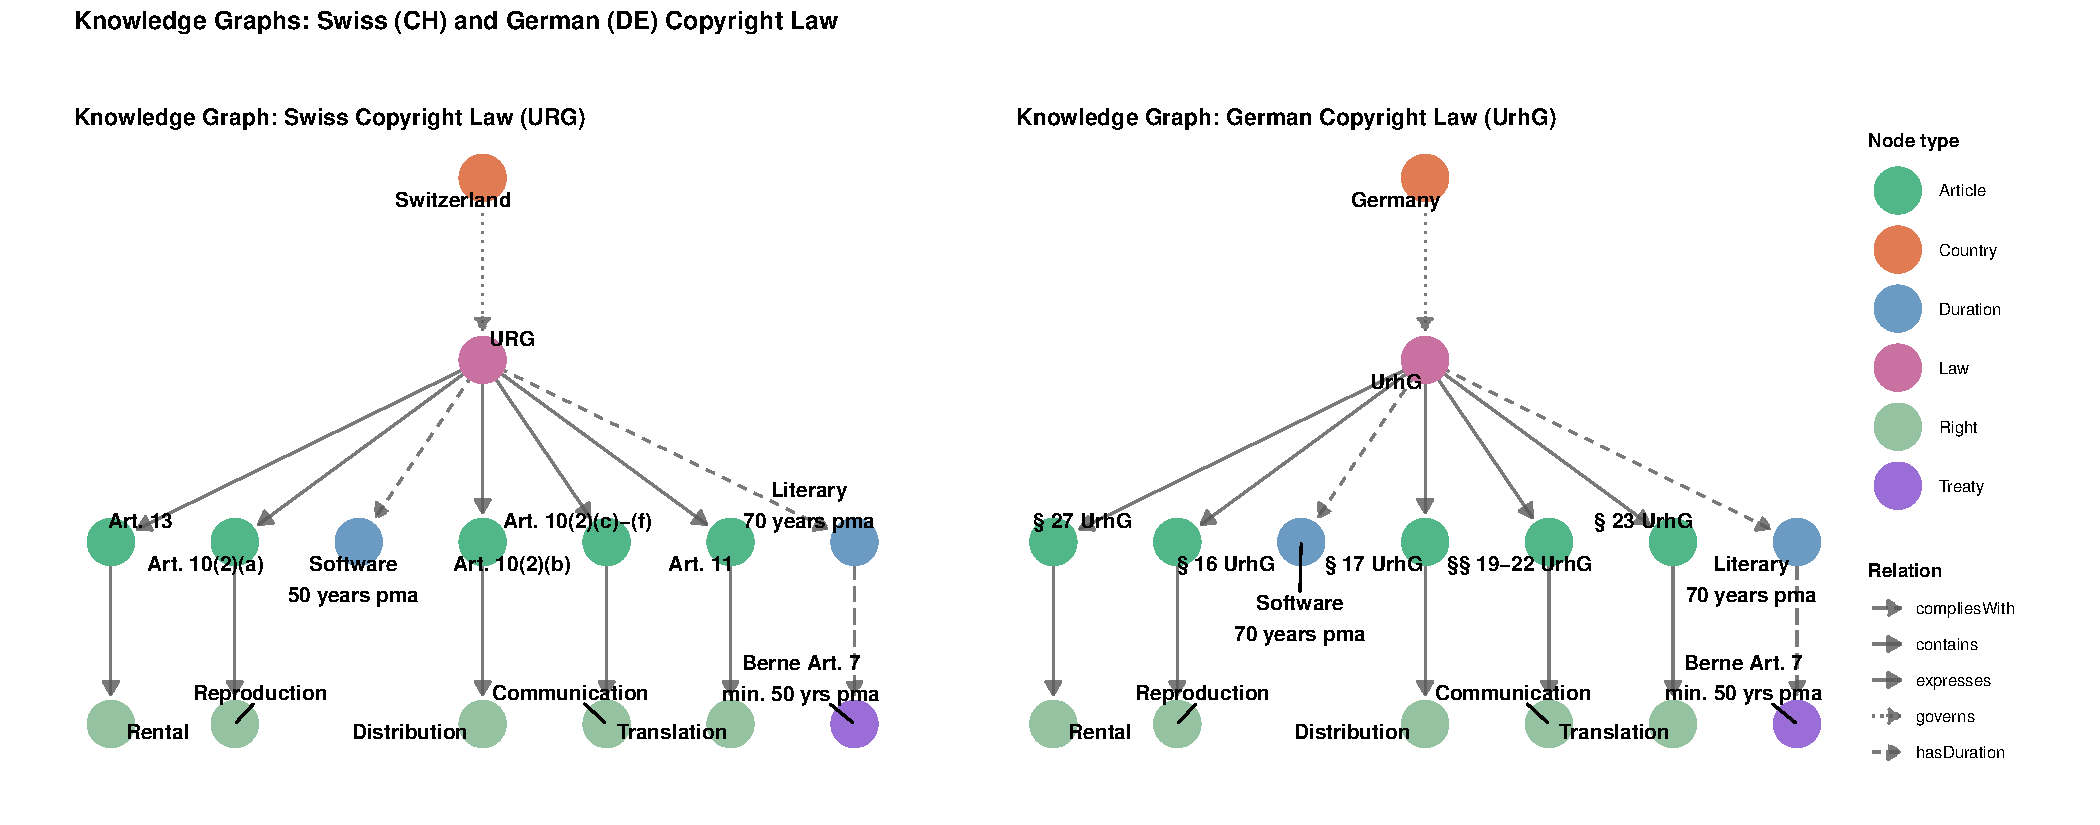
\includegraphics[width=0.97\textwidth]{kg_ch_de.pdf}}
  \caption{Knowledge graphs for Swiss and German copyright law.}
  \label{fig:kg}
\end{figure}

We store duration values as integers rather than text, which lets the
compliance checker compare them straight against the Berne minimum
without any parsing. If the jurisdiction comes back unknown, the system
falls back to a Berne Convention evidence record and says so to the user
rather than guessing.

\subsection{Stage 3: AKN Passage Extraction (Symbolic)}

The article reference from the KG (e.g.,\ ``Art.~29 URG'') is used to
locate the corresponding provision in the AKN XML file. The system
renders the relevant article as styled HTML with the supporting text
highlighted. It handles the different structural conventions used across
the nine corpora. AKN files are read at query time only and are not
loaded into the KG.

\subsection{Stage 4: Authentic Source Attribution (Symbolic)}
\label{sec:frbr}

Every AKN document embeds FRBR metadata that pins down both the
legislation and the version in force on a given date. We read four fields
out of it. The Work URI is the law's canonical identifier; in
the UI it becomes a clickable ``Official Source'' link straight to the
government portal, e.g.\ \href{https://www.legislation.gov.uk/ukpga/1988/48}%
{legislation.gov.uk} for the UK CDPA. Alongside it, the
applicability date records which version was in force at the
queried moment, the ELI URI carries the standardised European
identifier where one exists (Italy and Switzerland, in our corpus), and
the authenticity flag tells the user whether the document is the
official, legally binding text.

All four fields are stored in the KG at build time and returned in every
API response. The document viewer shows them as colour-coded badges:
green for authenticated sources, blue for the applicability date.

\subsection{Stage 5: Point-in-Time Navigation (Symbolic)}
\label{sec:pit}

Italy is the only jurisdiction for which multiple historical versions of
the copyright act are available as AKN files: 68~versions of
\emph{Legge}~633/1941 from 1941 to December~2025, sourced from the
Normattiva repository. The system builds an index of these versions and
returns the one in force at any user-specified date. In the UI, a date
picker appears for Italian documents. Selecting a date reloads the
correct historical version and updates all source attribution badges
accordingly.

\subsection{Stage 6: Answer Generation and Compliance Checker}

Stage~6 splits in two, one neural and one symbolic. For Q\&A queries (6a,
neural), the KG evidence, the passage, article reference, document title,
and FRBR Work URI, is serialised and handed to the LLM with a
grounding-focused prompt that constrains it to two to four sentences citing
the article. For compliance queries (6b, symbolic), no LLM is involved at
all: the checker reads the copyright duration for the queried country and
the Berne minimum straight from the KG, computes the margin, and returns a
structured verdict.

% ── 4. Implementation ───────────────────────────────────────────────────
\section{Implementation}

The system is a Flask web application with two UI modes: Q\&A and
Compliance Check, accessible via tab switching. The right panel is a
shared document viewer rendering AKN HTML, the FRBR meta bar, and, for
Italian documents, the point-in-time date picker.

\begin{table}[H]
\centering
\caption{Technology stack.}
\label{tab:stack}
\begin{tabularx}{\textwidth}{lX}
\toprule
\textbf{Component} & \textbf{Technology} \\
\midrule
Web framework      & Flask (Python~3.12) \\
KG store           & rdflib~7 (in-memory, TTL serialisation) \\
XML parsing        & lxml \\
LLM                & OpenRouter API (Gemini~2.0~Flash) \\
Schema validation  & Pydantic~v2 \\
Legal documents    & AKN XML (9~jurisdictions; 68~IT versions) \\
Ontology           & IPROnto OWL~\cite{delgado2003} \\
FRBR extraction    & \texttt{scripts/akn\_metadata.py} \\
Temporal index     & \texttt{scripts/point\_in\_time.py} \\
\bottomrule
\end{tabularx}
\end{table}

The KG is built on first request from a curated CSV dataset (9~rows, one
per jurisdiction) and then cached in memory. FRBR metadata triples get
embedded at build time through \texttt{akn\_metadata}, which brings the
graph to 446 triples in total.

\begin{figure}[H]
  \centering
  \begin{subfigure}[t]{0.47\textwidth}
    \centering
    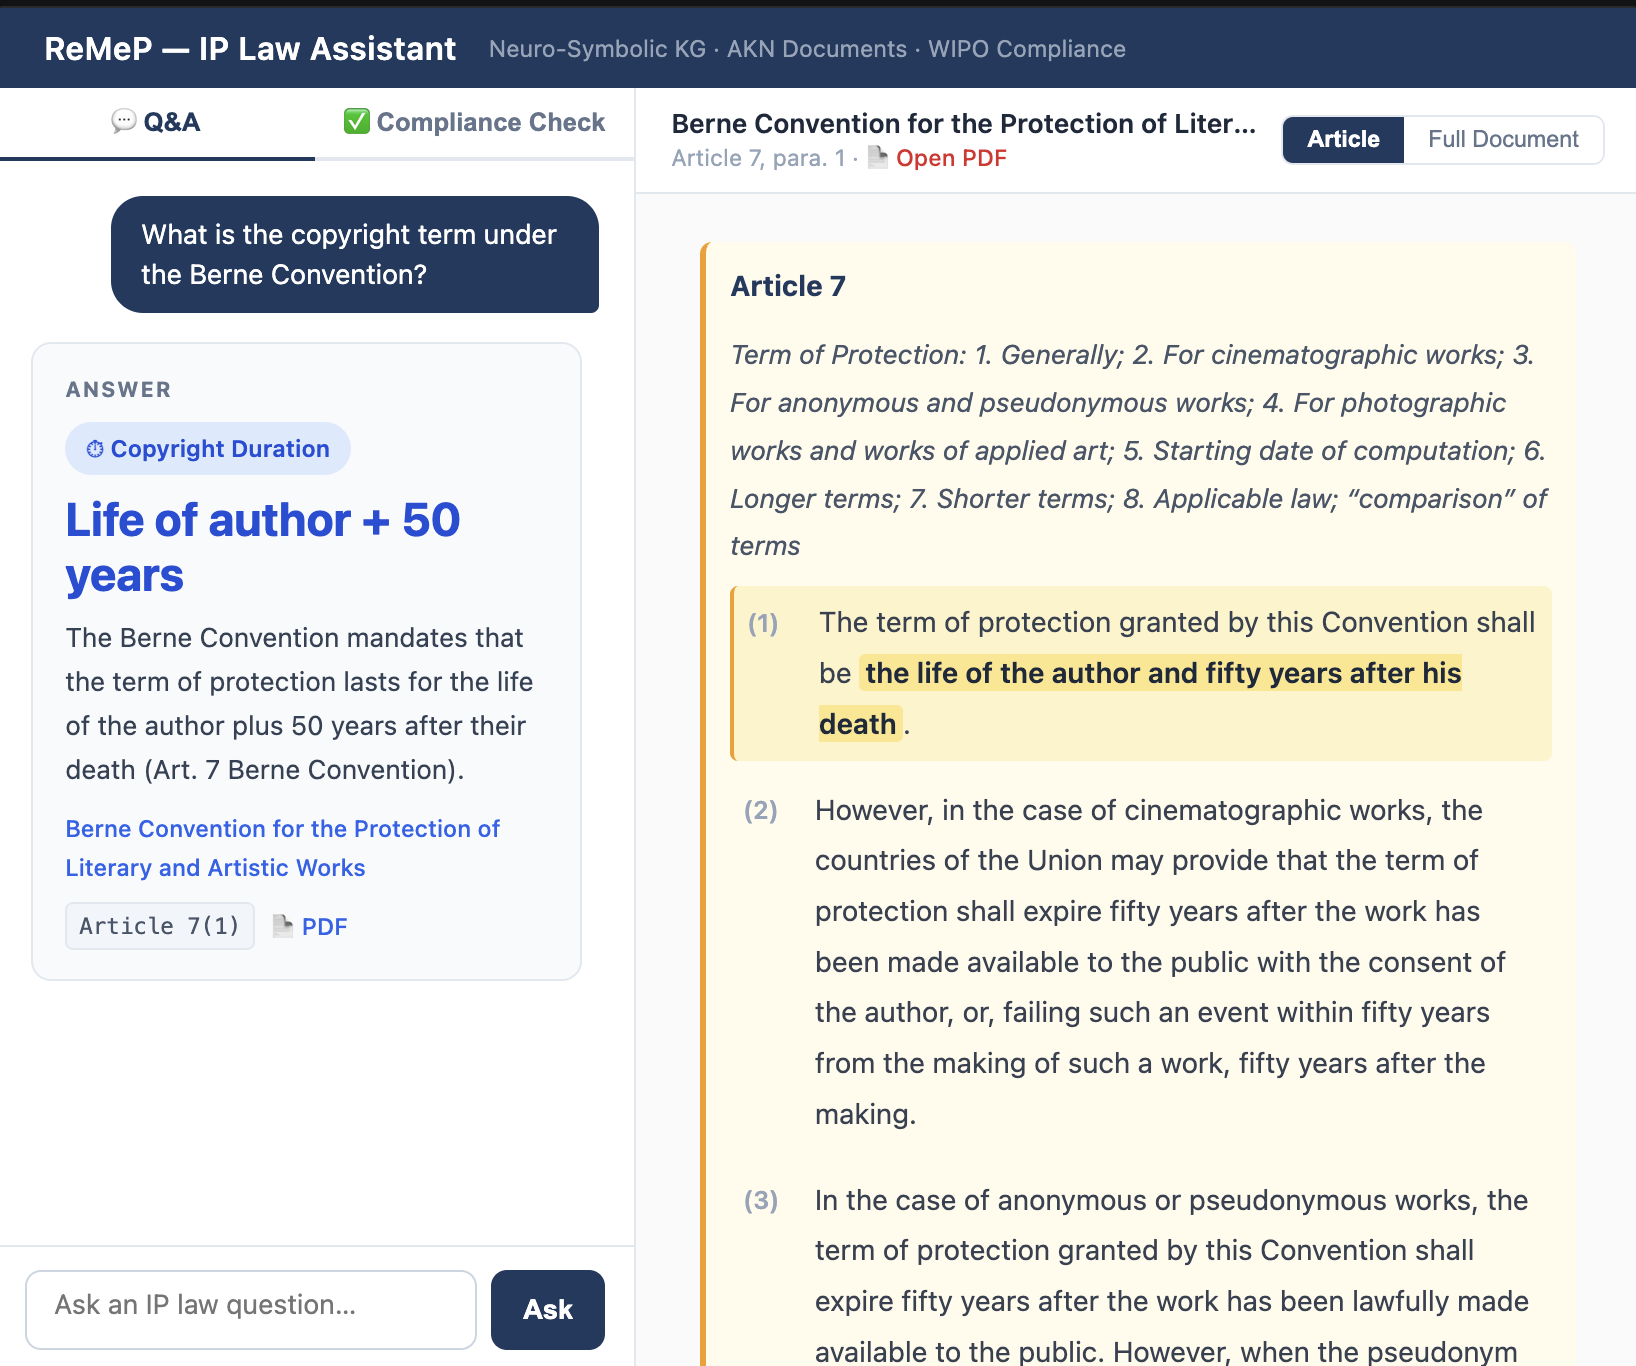
\includegraphics[width=\textwidth]{screenshot_qa.png}
    \caption{Q\&A mode: answer card with citation, AKN article
    rendered with highlighted supporting span, and FRBR meta bar
    (authenticity badge, applicability date, official-source link).}
  \end{subfigure}
  \hfill
  \begin{subfigure}[t]{0.47\textwidth}
    \centering
    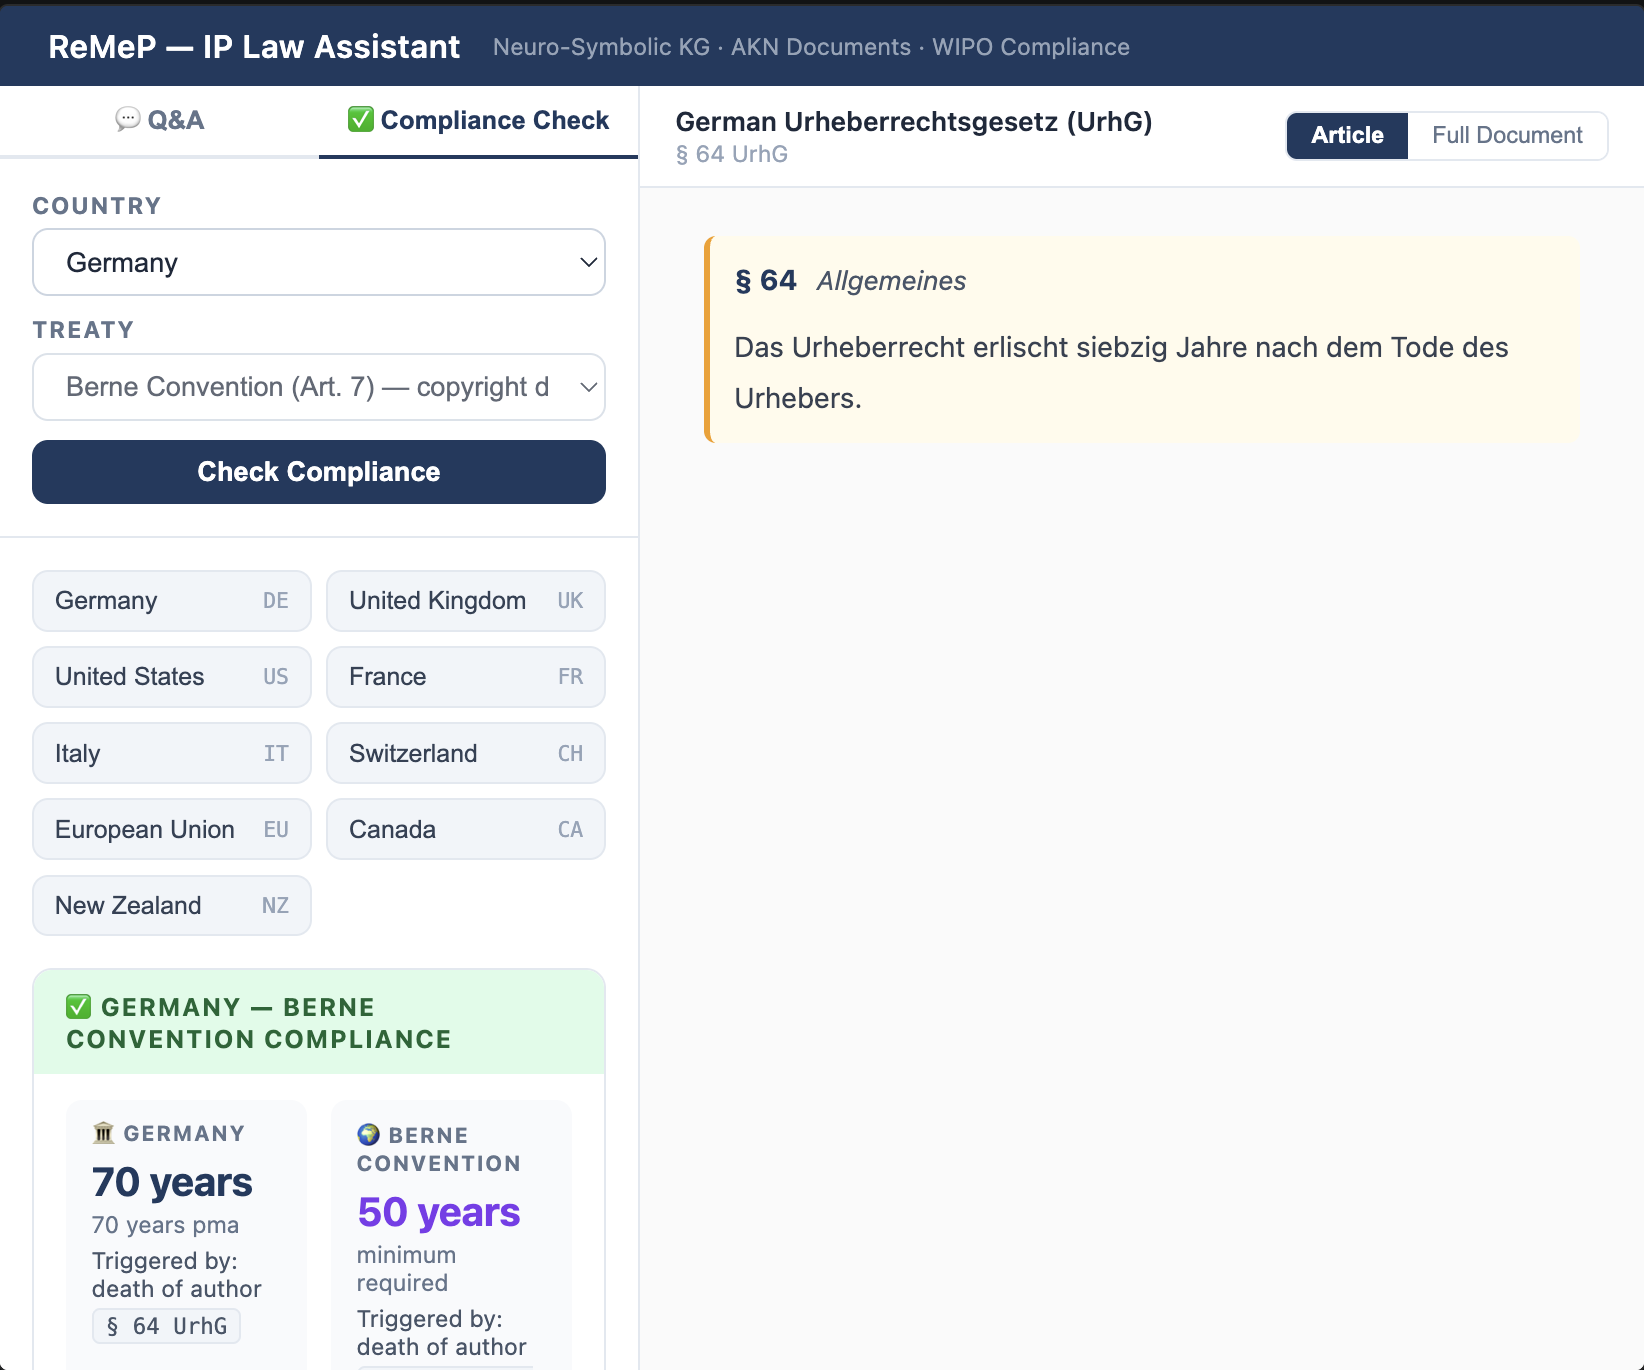
\includegraphics[width=\textwidth]{screenshot_compliance.png}
    \caption{Compliance Check mode: side-by-side comparison of national
    copyright duration vs.\ Berne Convention minimum, with verdict
    and margin in years.}
  \end{subfigure}
  \caption{The system UI in Q\&A and Compliance Check modes.}
  \label{fig:screenshots}
\end{figure}

% ── 5. Evaluation ───────────────────────────────────────────────────────
\section{Evaluation}

We tested the system along the same four dimensions it was built around.
On the question-answering side, queries in Italian, English, French, and
German are enriched correctly and routed to the right jurisdiction and
rule type, and we verified the AKN passage extraction against all nine
corpora, covering both \texttt{<article>} and \texttt{<section>} provision
types. The grounded answers always cite the article reference that came
from KG evidence, never one the LLM produced from memory.

Compliance checking illustrates the main advantage of the symbolic layer: the verdict is derived entirely from structured legal facts and explicit comparison rules rather than generated text. All nine
jurisdictions come back with the correct verdict (Table~\ref{tab:compliance}).
New Zealand, sitting at exactly 50~years, is classified as compliant with a
zero margin, and every 70-year jurisdiction as compliant with twenty years
to spare. The margin is computed in under 20\,ms, with no LLM in the loop.

\begin{table}[H]
\centering
\caption{Berne Convention Art.~7 compliance results (9~jurisdictions).}
\label{tab:compliance}
\begin{tabularx}{\textwidth}{lXccc}
\toprule
\textbf{Code} & \textbf{Jurisdiction} &
\textbf{Duration} & \textbf{Margin} & \textbf{Verdict} \\
\midrule
CA & Canada           & 70 years \emph{pma} & $+$20 & \textcolor{green!60!black}{Compliant} \\
EU & EU Directive     & 70 years \emph{pma} & $+$20 & \textcolor{green!60!black}{Compliant} \\
FR & France           & 70 years \emph{pma} & $+$20 & \textcolor{green!60!black}{Compliant} \\
DE & Germany          & 70 years \emph{pma} & $+$20 & \textcolor{green!60!black}{Compliant} \\
IT & Italy            & 70 years \emph{pma} & $+$20 & \textcolor{green!60!black}{Compliant} \\
NZ & New Zealand      & 50 years \emph{pma} & $0$    & \textcolor{green!60!black}{Compliant} \\
CH & Switzerland      & 70 years \emph{pma} & $+$20 & \textcolor{green!60!black}{Compliant} \\
UK & United Kingdom   & 70 years \emph{pma} & $+$20 & \textcolor{green!60!black}{Compliant} \\
US & United States    & 70 years \emph{pma} & $+$20 & \textcolor{green!60!black}{Compliant} \\
\bottomrule
\end{tabularx}
\end{table}

Source attribution holds up across the board: FRBR Work URIs are extracted
and rendered for all nine corpora. The authenticity flags vary by
jurisdiction, since the underlying metadata does: the UK marks its text
\texttt{FRBRprescriptive}, Switzerland and Italy use
\texttt{FRBRauthoritative}, and the rest leave it absent. ELI URIs show up
only for Italy and Switzerland. Point-in-time navigation, finally, resolves
the Italian versions correctly across the whole 1941--2025 span, and it does
so to the day: asking for 1973-05-30 returns V5 (in force since 1955-01-27),
while 1973-06-01 returns V6 (in force since 1973-05-31), one version later.

% ── 6. Limitations ──────────────────────────────────────────────────────
\section{Limitations and Future Work}

The system has clear limits, and the most interesting ones are not bugs but
open questions about how far the symbolic layer can be pushed. The biggest is
temporal grounding. Point-in-time navigation today works at the document
level: when the user picks a date, we swap in the whole AKN expression that
was in force then. The knowledge graph itself, though, knows nothing about
time, since its triples carry no \texttt{valid\_from} or \texttt{valid\_until}
markers. Adding that validity and querying it, would let the graph answer a question like ``Was France compliant on
1995-01-01?'' on its own, rather than by reloading a document. 

The remaining limits are less about ideas and more about reach. The current
graph is small by design: three rule types across nine jurisdictions, so
twenty-seven core nodes, hand-curated for the hackathon. A real system would
need automatic AKN-to-RDF ingestion covering a larger set of IPROnto dimensions, fed from live sources such as EUR-Lex or national gazette APIs.


% ── 7. Conclusion ───────────────────────────────────────────────────────
\section{Conclusion}

The worry with putting an LLM anywhere near legal compliance work is that you trade away explainability and transparency for fluency. What this prototype shows is that you do not have to. By pairing the LLM with a knowledge graph, we keep the model where it is genuinely useful, understanding a multilingual question and phrasing an answer, while every claim that carries legal weight comes from somewhere we can point to. The compliance verdict never touches the LLM at all: it is computed symbolically, straight from the knowledge graph, so there is nothing for the model to get wrong. FRBR/ELI source attribution and point-in-time navigation over the 68-version Italian corpus do the rest, tying each answer to a specific, dated, official provision rather than to ``the law'' in the abstract.

The combination we find most promising is the one this prototype only begins to exploit: a knowledge graph that holds both national legislation and the international obligations it has to meet. Setting the two side by side, and letting the symbolic layer check one against the other, seems to us a direction worth pursuing well beyond copyright duration. 


Source code is available at:
\url{https://github.com/Stocastico96/ReMeP_Hackathon_26}

% ── References ──────────────────────────────────────────────────────────
\newpage
\begin{thebibliography}{99}

\bibitem{palmirani2011}
M.~Palmirani and F.~Vitali.
\newblock Akoma-Ntoso for legal documents.
\newblock In \emph{Legislative XML for the Semantic Web}, pages 75--100.
  Springer, Dordrecht, 2011.
\newblock \url{https://doi.org/10.1007/978-94-007-1887-6_5}

\bibitem{ifla1998}
IFLA Study Group on the Functional Requirements for Bibliographic Records.
\newblock \emph{Functional Requirements for Bibliographic Records (FRBR)}.
\newblock IFLA, M\"{u}nchen, 1998.

\bibitem{eli2012}
Publications Office of the European Union.
\newblock European Legislation Identifier (ELI).
\newblock \emph{Official Journal of the EU}, 2012/C~325/02, 2012.
\newblock \url{https://eur-lex.europa.eu/eli-register/about.html}

\bibitem{delgado2003}
J.~Delgado, I.~Gallego, S.~Llorente, and R.~Garc\'{\i}a.
\newblock {IPROnto}: An ontology for intellectual property rights.
\newblock Distributed Multimedia Applications Group (DMAG), Universitat
  Polit\`{e}cnica de Catalunya, 2003.
\newblock \url{http://dmag.ac.upc.edu/ontologies/ipronto.owl}

\bibitem{palmirani2011lrml}
M.~Palmirani, G.~Governatori, A.~Rotolo, S.~Tabet, H.~Boley, and A.~Paschke.
\newblock {LegalRuleML}: {XML}-based rules and norms.
\newblock In \emph{RuleML 2011}, volume 6826 of \emph{LNCS}, pages 298--312.
  Springer, 2011.

\bibitem{nardi2026}
D.~Nardi et al.
\newblock An analysis of ontologies for the intellectual property domain.
\newblock In \emph{Proceedings of IRIS~2026} (this volume), 2026.

\bibitem{hitzler2022}
P.~Hitzler and M.~K.~Sarker.
\newblock \emph{Neuro-Symbolic Artificial Intelligence: The State of the Art}.
\newblock IOS Press, Amsterdam, 2022.

\bibitem{huang2023}
L.~Huang et al.
\newblock A survey on hallucination in large language models: Principles,
  taxonomy, challenges, and open questions.
\newblock arXiv:2311.05232, 2023.

\bibitem{oasis2018}
OASIS.
\newblock Akoma Ntoso Version 1.0.
\newblock OASIS Standard, 2018.
\newblock \url{http://docs.oasis-open.org/legaldocml/akn-core/v1.0/}

\bibitem{berne1886}
WIPO.
\newblock Berne Convention for the Protection of Literary and Artistic Works,
  Art.~7.
\newblock WIPO, Geneva, 1886 (as amended 1979).
\newblock \url{https://www.wipo.int/treaties/en/ip/berne/}

\end{thebibliography}

\end{document}